\chapter{Platform administration}\label{chap:PlatformAdministration}

%==================================================================
%================== PRIMERA SECCI�N ===============================
%==================================================================


\section{Custom Installation } \label{sec:custom}
The custom type installation   allows selecting or un-selecting individually packages to be install in the system. 
If any of the following software have been installed in the system \footnote{ The installation of any of these software components can cause conflicts in the system if already they exists.}, it is necessary to unselect these packages for installation. Once the installation process finished, the instructions cited here per each particular software must be followed.
\begin{itemize}
\item \textbf{MySQL}

In order to work correctly with \textsc{Thomas}, it is necessary to add a new user called ``thomas'' and to create the \textsc{Thomas} schema in the MySQL database. The following command must be executed:

\begin{verbatim}
$ cd ~/Magentix2/bin/MySQL
$ sh Import-ThomasDB.sh [MYSQL_ROOT_PASS]
\end{verbatim}

This command creates:
\begin{itemize}
 \item User ``thomas'' with password ``thomas''.
\item \textsc{Thomas} schema. This contains all database tables and relationships needed for the \textsc{Thomas} system.
\end{itemize}

\item  \textbf{Apache Tomcat}
To configure Apache Tomcat to work properly with Magentix2, it is needed to move the content from the \textsc{Thomas} directory to the current \textit{webapps/} tomcat directory:

\begin{verbatim}
$ cd ~/Magentix2/thomas
$ mv * /tomcat_directory/webapps
\end{verbatim}

\item \textbf{Apache Qpid}

The broker Qpid must be running in the system in order to connect agents:
\begin{verbatim}
$ cd $QPID_INSTALLATION
$ sbin/qpidd
\end{verbatim}


\end{itemize}

On the other hand, if any of these components  were installed during
the Magentix2 Desktop version installation, they would be configured as follows:
\begin{itemize}
\item \textbf{MySQL:}
	it would be installed in the directory \emph{mysql/}.

	By default, mysql root password is \textbf{mypassword}, this can be change in any moment.
\item \textbf{Apache Tomcat:}
	it would be installed in the directory \emph{apache-tomcat-7.0.4/} and 
	\textbf{8080} is the port configured to receive services petitions.

	The Catalina.out is a log for tomcat, it can be found in log tomcat directory.
\item  \textbf{Apache Qpid:}
      it would be installed in the directory \emph{/opt/qpid/} and
      \textbf{5672 } is the port configured to receive connections.

\end{itemize}



\subsection{Magentix2 installation description}

The following folders are created in the selected installation directory (by default \textit{\~{}/Magentix2}) both when full or  custom installation mode is selected ( depending on the selected packages):

\begin{itemize}
\item \textbf{bin/} 
 includes the executable files and folders required to launch and start the platform and services.
  These are:
\begin{itemize}
 \item \textit{Start-Magentix.sh}: it launches services and base agents of the platform \footnote{Magentix2 is launched without security, to enabled security refer to section \ref{sec:DesktopWithSecurity}}. Execute this script is not necessary the first time,  because the installer program do it. 
\item \textit{Stop-Magentix.sh}: it stops services and agents of the platform.
\item \textit{Launch-MagentixAgents.sh}: it launches the Magentix2 base agents (OMS, SF, TM and bridge agents).
\item \textit{Stop-MagentixAgents.sh}: it stops the Magentix2 base agents.
\end{itemize}
This services can be managed separately, existing a subdirectory per each service.

\begin{itemize}
\item \textbf{MySQL/} start, stop and configure MySQL service scripts.
\item \textbf{Tomcat/} start and stop Apache Tomcat service scripts.
\item \textbf{Qpid/} start and stop Apache Qpid service.
\end{itemize}



 
\textbf{Note:} All the commands could been executed as follows:
\begin{verbatim}
$ cd  ~/Magentix2/bin or ~/Magentix2/bin/subdirectory
$ sh script_name.sh
\end{verbatim}

In addition, also the following sub-directories are included:
\begin{itemize}
 
\item \textbf{configuration/} sub-directory: includes the Settings.xml and loggin.xml configuration files, necessary to launch Magentix2 user agents.

\item \textbf{security/} sub-directory: includes all required files to launch Magentix2 in secure mode. 
 
\end{itemize}


\item \textbf{docs/}
 includes javadoc and the Magentix2 documentation in Pdf format.
\item \textbf{lib/}
 includes Magentix2 library an all additional libraries required by Magentix2. How to import this library in projects is explained in  section \ref{sec:devel1stAgent}.
\item \textbf{examples/}
 includes some examples of Magentix2 agents implementation.
\item \textbf{src/}
 includes Magentix2 sources.
\item \textbf{thomas/}
 includes all services required by \textsc{Thomas} and Magentix2 platform. It also includes an example of a user web service.
\end{itemize}
 





\subsection{Possible Errors}

If MySQL is already installed in system,  the system informs about it with this error message:

\begin{codigo}
    101124 16:20:15 mysqld_safe Logging to syslog.
    101124 16:20:16 mysqld_safe A mysqld process already exists
    bin/mysqladmin: connect to server at 'localhost' failed
\end{codigo}

Moreover, if the following log is showed and \textsc{/etc/mysql/} directory \footnote{If it exists, it is recommended to delete it.} not exists, then an unstable installation of MySQL is in system. In this case,   a new installation of MySQL is recommended.
In section \ref{sec:MySQL} is explained how to install MySQL manually and section \ref{sec:custom} explain how to import the \textsc{Thomas} schema in the current MySQL database.

\begin{codigo} 
    bin/mysqladmin: connect to server at 'localhost' failed
    error: 'Can't connect to local MySQL server through 
    socket '/tmp/mysql.sock' (2)'
    Check that mysqld is running and that the socket: 
    '/tmp/mysql.sock' exists!
    bin/mysqladmin: connect to server at 'ubuntu' failed

    error: 'Lost connection to MySQL server at 'reading initial
    communication packet', system error: 111'
    ERROR 2002 (HY000): Can't connect to local MySQL server 
    through socket '/tmp/mysql.sock' (2)
\end{codigo}

%==================================================================
%================== SEGUNDA SECCI�N ===============================
%==================================================================
\section{Apache Qpid} \label{sec:apacheQpid}
%Qpid broker is a main component of Magentix2. Probably the contents of this section are not necessary if Magentix2 have been installed  by means of the the desktop version and Qpid was selected to be installed. On the contrary, this section is stronger recommenced in the case it was not desired to install Qpid together with Magentix2, because how to install Qpid  is explained in this section. Apache Qpid can be downloaded from \url{http://qpid.apache.org/download.cgi}
Qpid broker is a main component of Magentix2. In this section is described how it can be installed, in case it was not desired to install Qpid together with Magentix2. Apache Qpid can be downloaded from \url{http://qpid.apache.org/download.cgi}


The   following   libraries   must   be   installed   before   building   the   source distribution of Qpid:
\begin{itemize}
\item libboost�iostreams 1.35�dev: \url{http://www.boost.org} (1.35)
\item  e2fsprogs: \url{http://e2fsprogs.sourceforge.net/} (1.39)
\item pkgconfig: \url{http://pkgconfig.freedesktop.org/wiki/} (0.21)
\item uuid 1.2�1.41.4
\item ruby 4.2
\item ruby 1.8
\end{itemize}
In  Ubuntu  operating   systems  these   packages   can   be   installed   using   the 
Synaptic package management tool, but any other package manager might be 
valid. As an example, figure \ref{img:qpid1} shows how to install the libboost�iostreams 
1.35�dev library. 
\begin{figure}
\centering
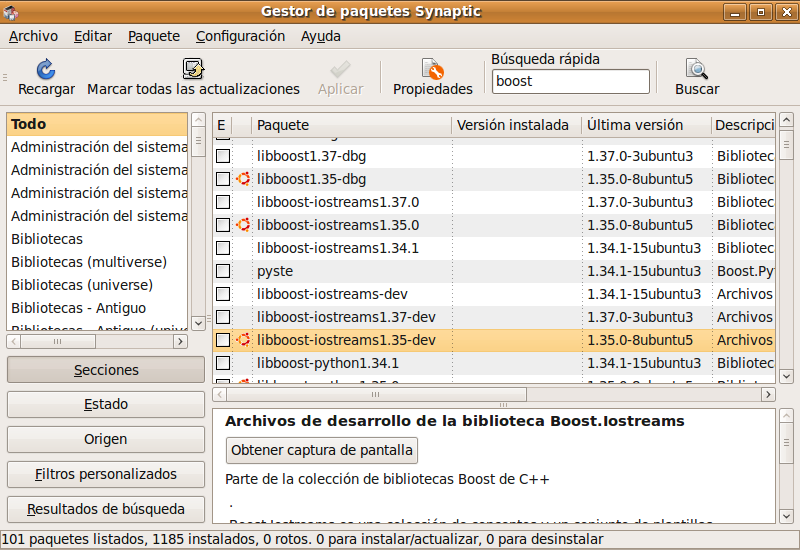
\includegraphics[scale=0.45]{Administration/images/qpid1}
\caption{Installing libboost�iostreams 1.35�dev library with Synaptic tool}
\label{img:qpid1}
\end{figure}
Once all the required libraries have been installed \footnote{ To install a Qpid version with security support, please follow at this section \ref{sec:QpidWithSecurity}}, Qpid broker can be downloaded from: \url{http://qpid.apache.org/download.cgi}. To install Qpid the following steps must be performed:
\begin{itemize}
 \item Uncompressing the donwloaded Qpid file.
 \item  \texttt{\$ ./configure --prefix= /home/hyperion/qpid} $\rightarrow$ Using the ��prefix  option when configuring, the location where the Qpid binaries are installed can be specified (in this example case, /home/hyperion/qpid).
 \item \texttt{\$ make install}
\end{itemize}

After a successful installation Qpid can be launched executing the following command inside the folder where Qpid was installed (in this example case, /home/hyperion/qpid): \texttt{\$ ./qpidd}.

Some values Qpid broker set by default are used by some components of Magentix2, therefore if any of them is changed, it is possible that the Settings.xml file has to be also modified. This file can be found in the configuration directory of Magentix2 distribution folder. Specifically the parameters that affect Qpid configuration in the Settings.xml file are the following:
\begin{codigo}
<entry key="host">localhost</entry>
<entry key="port">5672</entry>
<entry key="vhost">test</entry>
<entry key="user">guest</entry>
<entry key="pass">guest</entry>
<entry key="ssl">false</entry>
\end{codigo}

For example, if the port which Qpid broker is listening to is modified from the default 5672 to 5671, this change has to be also made on the Settings.xml file.

For those looking to adjust the Qpid broker operation there are plenty of advanced configuration options, for further information, please, refer to: \url{http://qpid.apache.org/books/0.7/AMQP-Messaging-Broker-CPP-Book/html/index.html}. Please note that if two ore more Qpid brokers have to work federated, a link between all the broker's amq.topic exchange has to be added.

%==================================================================
%================== TERCERA SECCI�N ===============================
%==================================================================
\section{MySQL}\label{sec:MySQL}
MySQL is a main component of the \textsc{Thomas} framework. This section explains how to properly configure MySQL to work in conjunction with \textsc{Thomas}. If MySQL was installed during the Magentix2 Desktop version installation, it will not be necessary to follow the steps shown here. However, if it was not installed together with Magentix2 or MySQL was already installed on the system, then this section helps to configure MySQL properly.


All   the   information   about   the  organizations  created with the \textsc{Thomas} framework and running on the Magentix2 platform  
is  permanently  stored   in a MySQL database. It is possible to create the  database schema and the user  employed by the \textsc{Thomas} framework  in MySQL by means of the the execution of the script \textit{Import-ThomasDB.sh}. This script is located in the directory \verb|/bin/MySQL|, which can be found into the Magentix2 installation folder. The commands needed to execute this script are the following (from the Magentix2 root directory):


\begin{verbatim}
$ cd bin/MySQL
$ sh Import-ThomasDB.sh [MYSQL_ROOT_PASS]
\end{verbatim}

However, it is also possible to create the \textsc{Thomas} database infrastructure step by step, without using the cited script. In this case, it is necessary to load into MySQL the   complete   structure   of   the   database from the \textit{Thomas.sql} file. This file is also located into the directory  \verb|/bin/MySQL|. In order to load this file,  the \textit{MySQL Administrator} tool should be opened,  and then  the \textit{Restore Backup} option must be selected, choosing the \textit{Thomas.sql} backup file to be restored. An example of this procedure can be shown in the figure \ref{img:mysql1}  

\begin{figure}[!h]
\centering
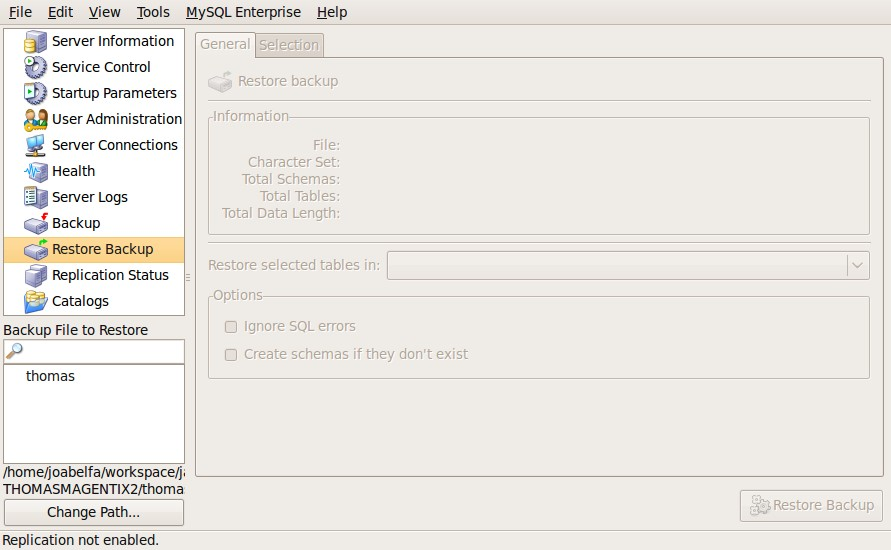
\includegraphics[scale=0.45]{Administration/images/mysql1}
\caption{Restoring the \textit{Thomas.sql} backup file in the \textit{Restore Backup} option of the \textit{MySQL Administrator}}  
\label{img:mysql1}
\end{figure}

The next required step is to add a new user to the \textsc{Thomas} schema in the \textit{User Administration} option of the \textit{MySQL Administrator} tool (see Figure \ref{img:mysql2}). The required fields must be fulfilled with the following information:

\begin{verbatim}
User=thomas
Password=thomas
\end{verbatim}

\begin{figure}[!h]
\centering
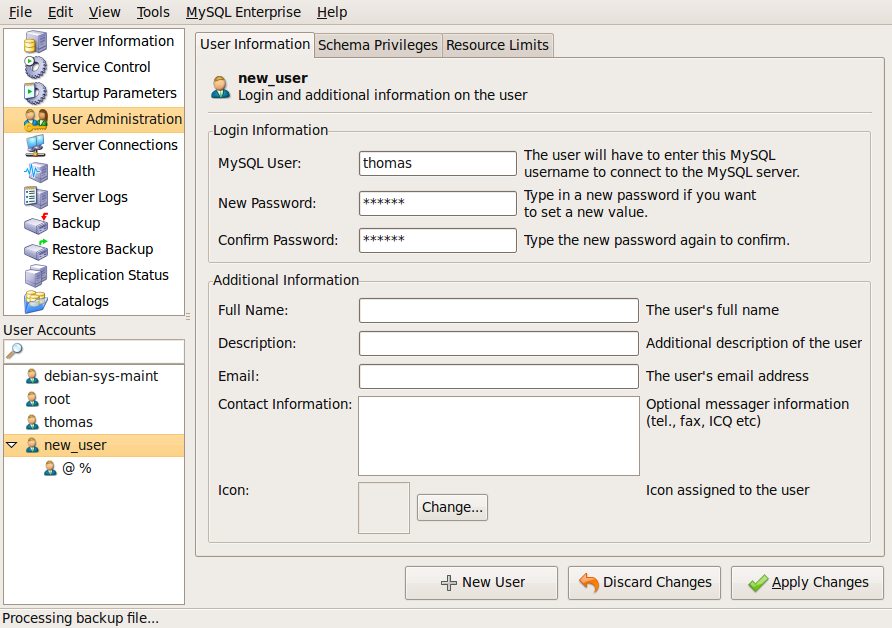
\includegraphics[scale=0.45]{Administration/images/mysql2}
\caption{Adding the necessary user information into the \textsc{Thomas} schema in the \textit{User Administrator} option of the \textit{MySQL Administrator} tool}
\label{img:mysql2}
\end{figure}

The \textit{ServerName}, \textit{databaseName}, \textit{userName} and \textit{password} entries must be also configured in the Settings.xml file located in the \verb|Magentix2/configuration| directory.
The parameters that affect MySQL configuration in the Settings.xml file are the following:

\begin{codigo}
<!-- Properties mysql -->
<entry key="serverName">localhost</entry>
<entry key="databaseName">thomas</entry>
<entry key="userName">thomas</entry>
<entry key="password">thomas</entry>
\end{codigo}

On the other hand, the THOMAS framework uses Apache Jena for manage the semantic description of the services.
In order to specify the required parameters for Jena, the Settings.xml file located in the \verb|Magentix2/configuration| directory
will be configured. The parameters that affect Jena configuration in the Settings.xml file are the following:
\begin{codigo}
<!-- Properties jena -->
<entry key="dbURL">jdbc:mysql://localhost/thomas</entry>
<entry key="dbType">MySQL</entry>
<entry key="dbDriver">com.mysql.jdbc.Driver</entry>
\end{codigo}

Check if the direction where agents OMS and SF are running is different host from where the MySQL is configured with the data base schema employed by the THOMAS framework.
If the OMS and SF are running in the same host, the configuration by default is correctly.

Finally, all available privileges for \textsc{Thomas} tables must be assigned to the \textit{thomas} user (Figure \ref{img:mysql4})
\begin{figure}[th!]
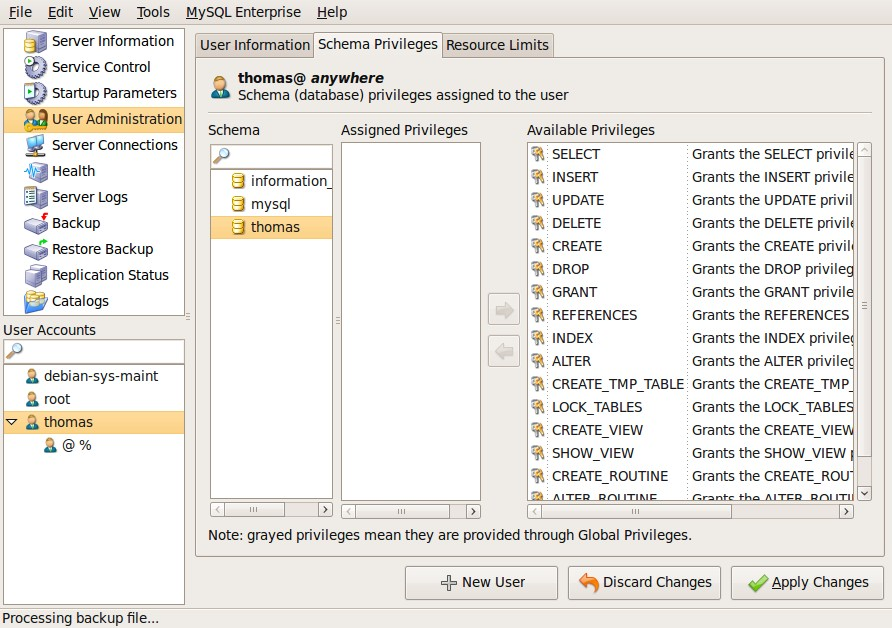
\includegraphics[scale=0.45]{Administration/images/mysql4}
\caption{Assigning privileges to the \textit{thomas} user in the \textit{User Administration} option of the \textit{MySQL Administration tool} }
\label{img:mysql4}
\end{figure}

%==================================================================
%================== CUARTA SECCI�N ================================
%==================================================================
\section{Apache Tomcat}
Apache Tomcat is a main component of Magentix2, because it allows to access to standard Java web services. If Apache Tomcat was installed during the Magentix2 Desktop version installation,  it will not be necessary to follow the steps shown here. On the contrary, in case Apache Tomcat was not installed together with Magentix2 or Apache Tomcat was already installed on the system, this section helps to configure it properly.

\textsc{Thomas}   platform   is   based   on   services (chapter \ref{chap:VirtualOrganizations}),   so   SF   and   OMS   service implementations have to be available as standard web services. Moreover, Magentix2 offers another service named MMS ( section \ref{sec:security}), which is responsible of controlling the user access to the platform.  This service must be also available as an standard web service. Any other user service (such as the application examples) need also to be available as standard web services. As mentioned above, Magentix2 uses Apache Tomcat to allow it. 


Apache Tomcat can be downloaded from: \url{http://tomcat.apache.org/}. The installation instructions can be found at: \url{http://tomcat.apache.org/tomcat-7.0-doc/setup.html}.

Once Tomcat is installed, packaged libraries of \textsc{Thomas} services (omsservices.war, sfservices.war)  have to be copied from \verb|Magentix2/thomas/| directory to the subdirectory\\ \verb|webapss/| of the Tomcat installation directory. Furthermore, the packaged library of the MMS service (MMS.war), which is also located at the  \verb|Magentix2/thomas/| directory, must  be  copied to the same \verb|webapss/|  subdirectory.

Then, the path where web services are deployed is required. In order to specify these parameters, the Settings.xml file
located in the Magentix2/configuration directory will be configured
The parameters that affect THOMAS configuration in the Settings.xml file are the following:
\begin{codigo}
<!-- Properties thomas -->
<entry key="OMSServiceDescriptionLocation">
	http://localhost:8080/omsservices/services/
</entry>
<entry key="SFServiceDescriptionLocation">
	http://localhost:8080/sfservices/services/
</entry>
\end{codigo}

Check if the direction where agents OMS and SF are running is different host from where the services (OMS and SF) are deployed, or if the port is different.
If the OMS and SF are running in the same host that  web services are deployed, the configuration by default is correctly.

In the same way, in order to run any developed web service from Tomcat, it is necessary to copy the packaged library (serviceName.war) to the subdirectory \verb|webapss/| of the Tomcat installation directory. In Magentix2 Desktop Version there is an example of a user web service, called \textit{SearCheapHotel}. It is possible to run this  example by means of coping the packaged library SearchCheapHotel.war (located at the \verb|Magentix2/thomas/| directory) to the subdirectory \verb|webapss/|  of Tomcat 



Once all the necessary services have been properly copied to the webapss directory, Tomcat can be started running the startup.sh file on the \verb|/bin/| subdirectory of the Tomcat installation directory.




\begin{figure}[!h]
\centering
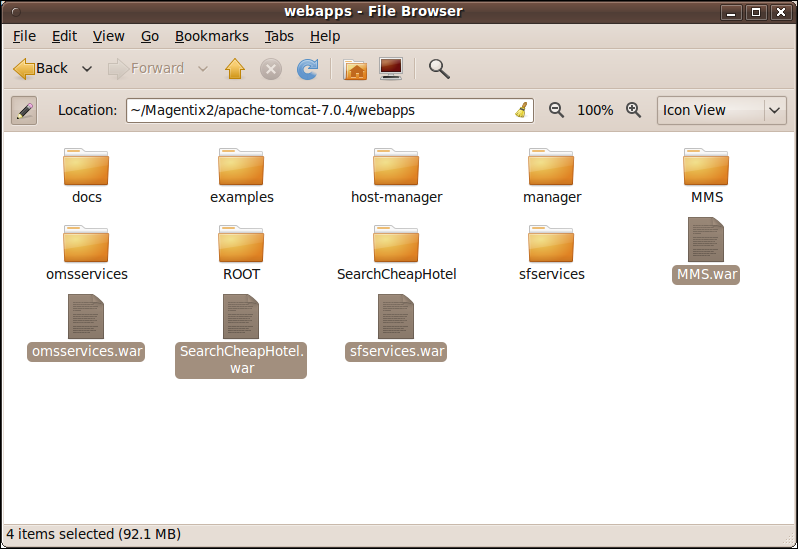
\includegraphics[scale=0.45]{Administration/images/tomcat1.png}
\caption{Location of web services files (*.war)}
\label{img:tomcat1}
\end{figure}



%==================================================================
%================== QUINTA SECCI�N ================================
%==================================================================
\section{Platform services}
This section explains how to launch platform agents without using the standard methods shown previously on this manual. This can be useful when some default parameters have been changed or if the platform runs in a distributed way.
\subsection{Running Bridge Agents}\label{sec:AdminRunningBridgeAgents}

Bridge agents are in charge of sending and receiving messages to or from foreign agents. For example, they allow Magentix2 agents to communicate with Jade agents. \textit{BridgeAgentInOut} manages messages that go from inside the platform to outside, whereas \textit{BridgeAgentOutIn} does the opposite. Bridge agents can be running on any host, they do not have to be in the same host where the QPid broker or other agents are running. A Java program has to be written and executed in order to launch bridge agents. The following code shows how to launch these agents:
\begin{lstlisting}
import es.upv.dsic.gti_ia.core.AgentsConnection;
import es.upv.dsic.gti_ia.core.AgentID;
import es.upv.dsic.gti_ia.core.BridgeAgentInOut;
import es.upv.dsic.gti_ia.core.BridgeAgentOutIn;

public class Main {
   public static void main(String[] args) throws Exception {
      AgentsConnection.connect();
      private BridgeAgentInOut inOutAgent;
      private BridgeAgentOutIn outInAgent;
      inOutAgent = new BridgeAgentInOut(new AgentID("BridgeAgentInOut"));
      outInAgent = new BridgeAgentOutIn(new AgentID("BridgeAgentOutIn"));
      inOutAgent.start();
      outInAgent.start();
   }
}
\end{lstlisting}
In the code shown above when the bridge agents are created (lines 11-12) they receive a new AgentID as argument. This new AgentID gets only one argument, the name of the agent. Platform agents, like bridge agents, must always have a well known name. For bridge agents the names must be: ``BridgeAgentInOut'' and ``BridgeAgentOutIn'' respectively.

In line 8 the connection of the agents to the platform is set using the method \texttt{AgentsConnec} \texttt{tion.connect()}. The parameters for this connection are specified in the configuration file \texttt{Settings.xml}. The method \texttt{AgentsConnection.connect()} should not be called if the platform security is enabled.
% 4 arguments, in order:
% \begin{enumerate}
%    \item Agent name: This argument cannot be modified. For the BridgeAgentInOut it must be ``BridgeAgentInOut'' and for BridgeAgentOutIn ``BridgeAgentOutIn''.
%    \item Agent protocol: This argument cannot be modified. For both agents it must be ``qpid''.
%    \item Agent host: Here we specify the ip address of the QPid broker we want to connect the agent to, in this specific example both agents connect to the broker running in the localhost, but we can specify other one, even it is possible to connect each bridge agent to a different QPid broker if these QPid brokers are federated.
%    \item Agent port: This is the port the QPid broker listens to. It has to match the port of the broker the agent connects to.
% \end{enumerate}

Once the agents have been created with the desired parameters, both are started (lines 13 \& 14). This Java program has to be manually executed when starting Magentix2 platform.

\subsection{Running OMS and SF Agents}
OMS and SF agents provide all the services of Thomas framework. These agents can be running on any host, they don't have to be in the same host where the QPid broker or other agents are running. A Java program has to be written and executed in order to launch OMS and SF agents. The following code shows how to launch these agents:

\begin{lstlisting}
import es.upv.dsic.gti_ia.architecture.Monitor;
import es.upv.dsic.gti_ia.core.AgentID;
import es.upv.dsic.gti_ia.core.AgentsConnection;
import es.upv.dsic.gti_ia.organization.OMS;
import es.upv.dsic.gti_ia.organization.SF;
import es.upv.dsic.gti_ia.core.AgentID;

public class Main {
   public static void main(String[] args) throws Exception {
      AgentsConnection.connect();
      OMS agentOMS = OMS.getOMS();
      SF agentSF = SF.getSF();
      agentOMS.start();
      agentSF.start();
   }
}
\end{lstlisting}

In the code shown above the agents OMS and SF are created (lines 11-12). The creation of these agents does not require any parameter.

% In the code shown above when the OMS and SF agents are created (lines 9-10) they receive a new AgentID as argument. This new AgentID gets 4 arguments, in order:

In line 10 the connection of the agents to the platform is set using the method \texttt{AgentsConnec} \texttt{tion.connect()}. The parameters for this connection are specified in the configuration file \texttt{Settings.xml}. The method \texttt{AgentsConnection.connect()} should not be called if the platform security is enabled. 
% 
% \begin{enumerate}
%    \item Agent name: This argument cannot be modified. For the OMS it must be ``OMS'' and for the SF ``SF''.
%    \item Agent protocol: This argument cannot be modified. For both agents it must be ``qpid''.
%    \item Agent host: Here we specify the ip address of the QPid broker we want to connect the agent to, in this specific example both agents connect to the broker running in the localhost, but it can be other one, even it is possible to connect each agent to a different QPid broker, if these QPid brokers are federated.
%    \item Agent port: This is the port the QPid broker listens to. It has to match the port of the broker the agent connects to.
% \end{enumerate}

Once the agents have been created with the desired parameters, both are started (lines 13 \& 14). This Java program has to be manually executed when starting Magentix2 platform.

%==================================================================
%================== SEXTA SECCI�N =================================
%==================================================================
\section{Configuring security} \label{sec:security}

\subsection{Introduction}


Figure  \ref{fig:magentix2security} shows an overview of the Magentix2 security infrastructure. Magentix2 Management Service (MMS) is a entity of Magentix2 that manages a part of the security of the platform (is located at the right of Figure \ref{fig:magentix2security}). In fact, MMS is responsible of  controlling the user accesses to the platform. Users will be present a certificate issued by a trusted third  party certificate authority (the red one in Figure \ref{fig:magentix2security}). Then, using the Magentix Certificate Authority (the blue one in Figure \ref{fig:magentix2security}), the MMS issues certificates for the agents (blue certificates in Figure \ref{fig:magentix2security}). Once an agent gets a valid certificate issued by the 
Magentix Authority Certificate, it can communicate to other agents in a secure way.

\begin{figure}[h!t]
	\centering
	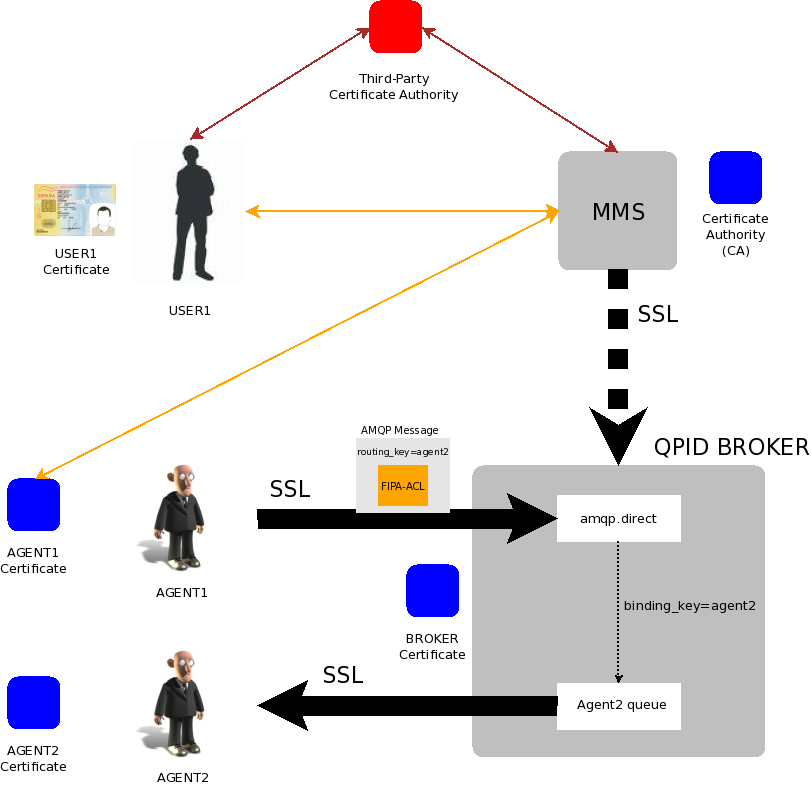
\includegraphics[width=0.5\textwidth]{Administration/images/magentix2-security.png}
	\caption{Magentix2 Security Infrastructure}
	\label{fig:magentix2security}
\end{figure}

The Magentix2 communication is based on AMQP standard. For supporting this standard, the Apache Qpid open source implementation is used.
So, the Qpid broker must be configured in order to support security. For this purpose, the broker will be use a certificate which issues for
the Magentix2 Certificate Authority. Thus,  agents in Magentix2 will  communicate with each other in a secure way using their agent certificates, which allow to authenticate with the Qpid broker. Furthermore, this broker  can also communicate with them using his certificate.


This section explains how to create the Magentix2 Certificate Authority and certificates for the Qpid broker and MMS. Moreover, how to configure MMS is also explained. Finally, it is explained how to install, configure and run the  Qpid broker with security support. 






\subsection{Supported features}

In order to ensure the security, the Magentix2 secure module supports the follow features:

\begin{enumerate}


 \item \textbf{Authentication:} The security module allows agents running on the Magentix2 platform to show other agents that effectively they are the agents they claim. This characteristic is the basis for all other features.


\item \textbf{Integrity:} The messages that one agent sends to another can not be manipulated by unauthorized agents while they are transmitted by the network.

\item \textbf{Confidentiality:} The messages sent thought the  network can not be accessible for unauthorized agents.

\item \textbf{Non-repudiation:} If an agent  receives a message of the agent B, the agent B is responsible for its message and can not negate a previous commitment or action.

\item \textbf{Privacy:} The owner of one agent which is executed in Magentix2 is not known by the rest of the agents of the platform, excepting the MMS. Therefore, the agents interact among them without know the user whom they represent.

\item \textbf{Accountability:} Although it offers privacy about the identities of the users whose agents run 
in Magentix2, the MMS saves a log with the relationship with the agents and the user owners. Therefore, if an agent realizes not desirable actions, his owner can be known and sanctioned as appropriate.

\item \textbf{Broker Resources Control:} The MMS is the unique entity that is authorized for administer the broker resources. The agents only are authorized to access to their queues.

\item \textbf{Control of the Interactions between Agents:} Using the ACL file of the Qpid broker, the MMS can restrict the communications between agents.
\end{enumerate}


\subsection{Using security in Magentix2 Desktop version} \label{sec:DesktopWithSecurity}


If Magentix2 has been installed by means of the desktop version, the security is disabled. To active the security in the system, these simple steps must be followed:



\begin{itemize}

 \item Executing MagentixPKI script. This script creates a public key infrastructure to support the Magentix Security Infrastructure. In order to customize the process, the steps of the section \ref{sec:creating} must be followed. The commands needed to execute the script are:
\begin{verbatim}
$ cd Magentix2/bin/security
$ sh MagentixPKI.sh CA_PASSWORD BROKER_PASSWORD MMS_PASSWORD
\end{verbatim}

\item Changing\footnote{If Magentix2 desktop installation directory is: \$HOME/Magentix2, and the passwords are the same of the script, only restart Qpid with security is necessary.} the passwords in the properties configurations (securityAdmin.properties and services.xml). How to configure these properties files is explained in section \ref{sec:MMS}. 

Some aspects must be considered before configure the  properties:
\begin{itemize}
	\item the \texttt{MMS\_PASSWORD} is the same to the key store and trust store.
  \item In the services.xml, only \texttt{MMS\_PASSWORD} is required.
  \item The \texttt{TOMCAT\_HOME} is \$HOME/Magentix2/apache-tomcat-7.0.4.
\end{itemize}


\item Adding a new trusted third party certificate authority (explained in section \ref{sec:AddthirdParty}).

\item Restarting the Tomcat service executing the commands:
\begin{verbatim}
$ cd Magentix2/bin/Tomcat
$ sh Stop-Catalina.sh
$ sh Start-Catalina.sh
\end{verbatim}

\item Stopping Qpid without security and restart \footnote{Qpid was executing on background.} with security, executing the commands:
\begin{verbatim}
$ cd ../Qpid
$ sh Stop-Qpid.sh 
$ sh Start-QpidWithSecurity.sh
\end{verbatim}

\end{itemize}

The following log is showed if the process has been done correctly:
\begin{codigo}
2010-12-17 13:18:24 notice Listening on TCP port 5672
2010-12-17 13:18:24 notice Listening for SSL connections
on TCP port 5671
2010-12-17 13:18:24 notice Read ACL file
 "../bin/security/broker.acl"
2010-12-17 13:18:24 notice Broker running
\end{codigo}

\subsection{Creating certificates} \label{sec:creating}

In this section, how to create\footnote{For this purpose, certutil (\url{http://www.mozilla.org/projects/security/pki/nss/tools/certutil.html}) and keytool (\url{http://download.oracle.com/javase/1.3/docs/tooldocs/win32/keytool.html}) commands are used.} a Magentix2 Public Key Infrastructure manually is explained. These steps can make a more custom configuration process (indicating  the type of
algorithm, duration of validity, etc.). The basic components that can be configured are:

\begin{itemize}
 \item Magentix Certificate Authority (MagentixCA).
 \item  Qpid broker.
 \item Magentix2 Management Service (MMS).
\end{itemize}




Firstly, it is recommended to create the PKI infrastructure in a new folder (but it is optional).

\begin{verbatim}
$ mkdir security
$ cd security 
\end{verbatim}

\subsubsection{Magentix Certificate Authority (MagentixCA)} \label{sec:MagentixCA}

The following steps show how to create  MagentixCA certificates.
\begin{itemize}

\item \textbf{Creating a new certificate database in the CA\_db directory :}
\begin{verbatim}
$ mkdir CA_db 
$ certutil -N -d CA_db 
\end{verbatim}

In this step, the password for CA is introduced. Afterwards, it will be referenced as \texttt{PASSWORD\_CA}.

\item \textbf{Creating a Self-signed Root CA certificate, specifying the subject name for the certificate (MagentixCA):}
\begin{verbatim}
$ certutil -S -d CA_db -n "MagentixTheCA" \
 -s "CN=MagentixCA,O=Magentix" -t "CT,," -x -2
\end{verbatim}

The \texttt{PASSWORD\_CA} is required. The system asks about same aspects, and the following answers must be proportioned: 

\begin{itemize}
 \item Typing ``y'' for ``Is this a CA certificate [y/N]?''
 \item Pressing enter for ``Enter the path length constraint, enter to skip [$<$0 for unlimited path]:``
 \item Typing ''n'' for ''Is this a critical extension [y/N]?''
\end{itemize}

   
\item \textbf{Extracting to a file the CA certificate from the CAs certificate database:}
\begin{verbatim}
$ certutil -L -d CA_db -n "MagentixCA" \
 -a -o CA_db/rootca.crt
\end{verbatim}

\end{itemize}

\subsubsection{Qpid broker}

A certificate identifies the broker, which will be signed by the Magentix CA. The following steps show how to create  Qpid certificates.
 \begin{itemize}

 \item \textbf {Creating a certificate database for the Qpid Broker:}
\begin{verbatim}
$ mkdir broker_db 
$ certutil -N -d broker_db
\end{verbatim}

In this step the password for the Qpid broker is introduced. Afterwards, it will be referenced as \texttt{PASSWORD\_BROKER}.


\item \textbf {Importing the CA certificate into the broker’s certificate database, and marking it trusted for issuing certificates for SSL client and server authentication:}
\begin{verbatim}
$ certutil -A -d broker_db -n "MagentixCA" -t "TC,," \
	   -a -i CA_db/rootca.crt
\end{verbatim}
The \texttt{PASSWORD\_BROKER} is required.

\item  \textbf {Creating the server certificate request, specifying the subject name for the server certificate.}
\begin{verbatim}
$ certutil -R -d broker_db -s "CN=broker,O=Magentix" \
	   -a -o broker_db/server.req 
\end{verbatim}
The \texttt{PASSWORD\_BROKER} is required.

Note that this step generates the server’s private key, so it must be done in the servers database directory. 

\item  \textbf {This step simulates the CA signing and issuing a new server certificate based on the servers certificate request:}
\begin{verbatim}
$ certutil -C -d CA_db -c "MagentixCA" \
  -a -i broker_db/server.req \
  -o broker_db/server.crt -2 -6 
\end{verbatim}

The new certificate is signed with the CAs private key, so this operation uses the CAs databases (The \texttt{PASSWORD\_CA} is required). For leaving the new certificates of the servers in a file the following actions must be performed: 


\begin{itemize}
 \item Selecting ``0 - Server Auth'' at the prompt
\item Pressing 9 at the prompt
\item Typing ``n'' for ``Is this a critical extension [y/N]?''
\item Typing ``n'' for ``Is this a CA certificate [y/N]?''
\item Entering ``-1'' for ``Enter the path length constraint, enter to skip [$<$0 for unlimited path]: $>$''
\item Typing ``n'' for ``Is this a critical extension [y/N]?''
\end{itemize}

\item  \textbf {Importing (adding) the new server certificate to the brokers certificate database in the server\_db directory with the broker nickname:}
\begin{verbatim}
$ certutil -A -d broker_db -n broker -a \
 -i broker_db/server.crt -t ",," 
\end{verbatim}

\item \textbf {Verifying if the certificate is valid:}

\begin{verbatim}
$ certutil -V -d broker_db -u V -n broker
\end{verbatim}
  At the end, the following message must be showed: certificate is valid.
  
\end{itemize}

\subsubsection{Magentix2 Management Service}\label{sec:mms}

This certificate identifies the MMS, which will be signed by the Magentix CA. In this section, how to create a new MMS keystore and trustore is explained. 


\begin{itemize}
   \item \textbf {Importing the CA certificate in to the trust store and import the CA certificate in to the key store (need for client authentication):}
\begin{verbatim}
$ keytool -import -trustcacerts -alias MagentixCA \
	-file CA_db/rootca.crt -keystore MMSkeystore.jks
$ keytool -import -trustcacerts -alias MagentixCA \
	-file CA_db/rootca.crt -keystore MMStruststore.jks
\end{verbatim}

In this step, the password for key store and trust store are introduced. Afterwards, will be referenced as \texttt{PASSWORD\_MMSKEYSTORE} and \texttt{PASSWORD\_MMSTRUSTSTORE}
respectively.

\item \textbf {Generating keys for the MMS certificate:}.
\begin{verbatim}
$ keytool -genkey -alias MMS -keyalg RSA\
        -dname "CN=MMS,O=Magentix" \
        -keystore MMSkeystore.jks
\end{verbatim}
Press enter when prompted for the password to select the same password as the key-store. 

\item \textbf{Creating a certificate request:}
\begin{verbatim}
$ keytool -certreq -alias MMS -keystore MMSkeystore.jks \
   -file mms.csr
\end{verbatim}
The \texttt{PASSWORD\_MMSKEYSTORE} is required.

\item \textbf{Signing the certificate request using CA certificate:}
\begin{verbatim}
$ certutil -C -d CA_db/ -c "MagentixCA" -a -i mms.csr \
 -o mms.crt
\end{verbatim}

The \texttt{PASSWORD\_CA} is required.

\item \textbf {Importing the certificate into the key store:}
\begin{verbatim}
$ keytool -import -trustcacerts -alias MMS -file mms.crt \
         -keystore MMSkeystore.jks
\end{verbatim}

The \texttt{PASSWORD\_MMSKEYSTORE} is required.

\end{itemize}

\subsection{Exporting the MMS certificate with the public Key} \label{sec:exportmmscertificate}

This command is used to export the MMS public key  into a file. It will be sent to users and they will must be imported into his trustores.
Thereby, the security context (mutual authentication) with the MMS and users will be created.

\begin{verbatim}
$ keytool -export -alias MMS -file mms.crt \
 -keystore MMSkeystore.jks
\end{verbatim}

The \texttt{PASSWORD\_MMSKEYSTORE} is required.

\subsection{Importing new trusted third party certificate authority} \label{sec:AddthirdParty}


The following command is used to import a new trusted third party certificate authority.
Thereby, all users with certificate issues by these trusted third party can be communicate in a security context (mutual authentication) with the MMS.




\begin{verbatim}
$ keytool -import -trustcacerts -alias FNMT \
  -file FNMTClase2CA.cer -keystore MMSkeystore.jks
\end{verbatim}

\emph{$<$alias$>$}: user name identifying

\emph{$<$file$>$}: certificate with user public key\footnote{For example, to accept users issues for the Fabrica Nacional de Moneda y Timbre (FNMT) download and import this certificate (\url{http://www.cert.fnmt.es/index.php?cha=cit\&sec=4\&page=139\&lang=es}).}.

The \texttt{PASSWORD\_MMSKEYSTORE} is required.



\subsection{Tracing Service}\label{sec:CertificatetracingService}

In the platform, only a user authorized can be launch a trace manager agent (TM) (explained in section \ref{sec:tracingService}), to avoid the supplanting of this user/agent. The functionality of MMS has been limited in order to not issue a certificates for a TM user.
Therefore, the certificate for  TM  agent will be created manually by means of the following steps:


\begin{itemize}

\item \textbf{Importing the CA certificate in to the key store (needed for client authentication):}
\begin{verbatim}
$ keytool -import -trustcacerts -alias MagentixCA  \
	  -file CA_db/rootca.crt -keystore keystore.jks
\end{verbatim}

The \texttt{PASSWORD\_USERKEYSTORE} is required.

\emph{$<$file$>$}: the rootca.crt. Section \ref{sec:MagentixCA}  shows how to obtain this file.

\item \textbf {Generating keys for the TM certificate:}
\begin{verbatim}
$ keytool -genkey -alias TM -keyalg RSA \
 -dname "CN=TM,O=Magentix" -keystore keystore.jks 
\end{verbatim}

Pressing enter when prompted for the password to select the same password as the key-store. 

The \texttt{PASSWORD\_USERKEYSTORE} is required.


\item  \textbf {Creating a certificate request:}
\begin{verbatim}
$ keytool -certreq -alias TM -keystore keystore.jks 
        -file tm.csr
\end{verbatim}

The \texttt{PASSWORD\_USERKEYSTORE} is required.
\item \textbf {Signing the certificate request using a CA certificate:}
\begin{verbatim}
$ certutil -C -d CA_db/ -c "MagentixCA" -a -i tm.csr \
         -o tm.crt
\end{verbatim}
The \texttt{PASSWORD\_CA} is required.

\item \textbf {Importing  the certificate into the key store:}
\begin{verbatim}
$ keytool -import -trustcacerts -alias TM -file tm.crt \
        -keystore keystore.jks 
\end{verbatim}
The \texttt{PASSWORD\_USERKEYSTORE} is required.

\end{itemize}

\subsection{Magentix2 Management System (MMS)} \label{sec:MMS}

The MMS is distributed as a war project (Web Application aRchive). In webapps directory, where it is deployed, exists a MMS folder. In this folder, the configuration files are located.

Once the certificate infrastructure has been created, the properties files will have to be configured correctly.
If the Magentix2 Desktop version has been installed, default options are correctly configured.

It should be remember that the root directory is \texttt{TOMCAT\_HOME/}bin. for the relative path 

\begin{itemize}
\item nss.cfg 

This file is in the folder: \texttt{TOMCAT\_HOME}/webapps/MMS/WEB-INF/classes/.

In this file, the path of Magentix2 Certificate Authority (CA\_db) is represented. Only change the 
\textit{nnsSecmondDirectory} if the CA\_db is in other path than Magentix2/bin/security, as it can be
shown in the following example (Figure \ref{fig:nns.cfg}).


\begin{figure}[h!]
\begin{codigo}
name = NSSkeystore
nssLibraryDirectory = /usr/lib
nssSecmodDirectory = ../bin/security/CA_db
nssModule = keystore
\end{codigo}
\caption{An example of the nss.cfg file.}
\label{fig:nns.cfg}
\end{figure}

\item services.xml

This file is in: \texttt{TOMCAT\_HOME}/webapps/MMS/WEB-INF/services/MMS/META-INF/.

In this file, the rampart properties are configured. The Figure \ref{fig:services.xml} shows an example of this file.

\begin{figure}[!h]
\begin{codigo}
<ramp:signatureCrypto>
  <ramp:crypto provider="org.apache.ws.security.components
     .crypto.Merlin">
     <ramp:property name="org.apache.ws.security.crypto
     .merlin.keystore.type">
	    JKS
     </ramp:property>
     <ramp:property name="org.apache.ws.security.crypto
     .merlin.file">
	    ../bin/security/MMSkeystore.jks
     </ramp:property>
     <ramp:property name="org.apache.ws.security.crypto
     .merlin.keystore.password">
	    MMS_PASSWORD
     </ramp:property> 
 </ramp:crypto>
</ramp:signatureCrypto>
\end{codigo}
\caption{An example of the services.xml file.}
\label{fig:services.xml}
\end{figure}

\item securityAdmin.properties

This file is in the directory: \texttt{TOMCAT\_HOME}/webapps/MMS/WEB-INF/classes/.

\begin{itemize}



\item Setting the path and password to MMS key and trust store\footnote{ How to create the MMS keystore and trustore was explained in section \ref{sec:mms}} (Figure \ref{fig:admin.properties1}). 

\begin{figure}[h!]
\begin{codigo}
<!-- Only MMS Administrator -->


# set the base path for accessing keystore user
KeyStorePath=../bin/security/MMSkeystore.jks
#set the password to keystore
KeyStorePassword=MMS_PASSWORD

# set the base path for accessing truststore user
TrustStorePath=../bin/security/MMStruststore.jks
#set the password to truststore
TrustStorePassword=MMS_PASSWORD

\end{codigo}
\caption{First section of the securityAdmin.properties file.}
\label{fig:admin.properties1}

\end{figure}

\item Changing the algorithm type for encryption and validity time (in days) for the certificates (Figure \ref{fig:admin.properties2}).

\begin{figure}[h!]
\begin{codigo}
#set the type of algorithm for the signature certificates
sigAlg=SHA1WithRSA
#set the validity time for the certificates (days)
Validity=90
\end{codigo}
\caption{Second section of the securityAdmin.properties file.}
\label{fig:admin.properties2}
\end{figure}

\item Setting the base path for accessing to the ACL broker  (Figure \ref{fig:admin.properties3}). 

\begin{figure}[h!]
\begin{codigo}
# set the base path for accessing to broker acl.
ACLPath=../bin/security/broker.acl
\end{codigo}
\caption{Third section of the securityAdmin.properties file.}
\label{fig:admin.properties3}
\end{figure}


\item Setting the base path for logging the registers User/Agent (Figure \ref{fig:admin.properties4}). By default, the path is \texttt{TOMCAT\_HOME}/logs.

\begin{figure}[h!]
\begin{codigo}
#set the base path for log the registers User / Agent.
Userlog=logs/MMSregisters.log
\end{codigo}
\caption{Fourth section of the securityAdmin.properties file.}
\label{fig:admin.properties4}
\end{figure}


\item Setting the properties for the Magentix Certificate Authority \footnote{The process to create Magentix CA was explained in section \ref{sec:MagentixCA}.} (Figure \ref{fig:admin.properties5}).

\begin{figure}[h!]
\begin{codigo}
#set the alias to root certificate
aliasCA=MagentixCA
#set the password to root nss db
password=PASSWORD_CA
#set the type to root nss db
type=PKCS11
\end{codigo}
\caption{Fight section of the securityAdmin.properties file.}
\label{fig:admin.properties5}
\end{figure}


\item Setting the base path for accessing to the configuration nss file (Figure \ref{fig:admin.properties6}).

\begin{figure}[h!]
\begin{codigo}
#set the base path for accessing to configuration file nss.
pathnsscfg=webapps/MMS/WEB-INF/classes/nss.cfg
\end{codigo}
\caption{Sixth section of the securityAdmin.properties file.}
\label{fig:admin.properties6}
\end{figure}


\item Setting the properties of the Qpid broker (Figure \ref{fig:admin.properties7}).

\begin{figure}[h!]
\begin{codigo}
#set the properties of qpid broker
host=localhost
port=5671
vhost=test
user=guest
pass=guest
ssl=true
saslMechs=EXTERNAL
\end{codigo}
\caption{Seventh section of the securityAdmin.properties file.}
\label{fig:admin.properties7}
\end{figure}


\item Setting the values of the certificates (Figure \ref{fig:admin.properties8}).
\begin{figure}[h!]
\begin{codigo}
#set the values of certificates
organizationalUnit=Magentix
organization=orgnization
city=city
state=state
country=ES
\end{codigo}
\caption{Eighth section of the securityAdmin.properties file.}
\label{fig:admin.properties8}
\end{figure}


\item Setting the Rampart configuration properties (Figure \ref{fig:admin.properties9}).
\begin{figure}[h!]
\begin{codigo}
#Rampart config: set the alias value of certificate for 
sign the messages.
alias=mms
#set the password of mmskeystore 
key=PASSWORD_MSSKEYSTORE 
\end{codigo}
\caption{Ninth section of the securityAdmin.properties file.}
\label{fig:admin.properties9}

\end{figure}

\end{itemize}
\end{itemize}


Tomcat must be restarted in order to update changes. Therefore, the following commands must be executed. If Magentix2Desktop is installed:
\begin{verbatim}
$ cd Magentix2/bin/Tomcat
$ sh Stop-Catalina.sh
$ sh Start-Catalina.sh
\end{verbatim}

In other cases:


\begin{verbatim}
$ cd TOMCAT_HOME/bin
$ sh ./shutdown.sh
$ sh ./startup.sh
\end{verbatim}



\subsection{Qpid broker with security support}
\label{sec:QpidWithSecurity}

\subsubsection{Installing}
In this section is explained how to install Qpid with security. If the Magentix2Desktop has been installed and Qpid was selected for install, it is not needed execute this step. In that case, it is only necessary to  execute the script bin/Qpid/Start-QpidWithSecurity.sh  in order to execute Qpid with security.

For installing the  Qpid dependencies,  please refer to the section \ref{sec:apacheQpid}. Once the basic dependencies are resolved, follow the next steps:
%seccionQpid hacer referencia a la seccion de instalación de Qpid (seccion 6.1)
\begin{enumerate}
	\item Installing the following libraries before building the source distribution of Qpid with security (SSL and SASL must be installed) :
		\begin{itemize}
			\item libnss3-1d
			\item libnspr-dev
			\item libnss3-dev
			\item libnss3-tools
			\item libsasl2-dev 
			\item sasl2-bin
	\end{itemize}
	
On Ubuntu operating systems these packages can be installed using the Synaptic package management tool, but any other package manager might be valid.


\item Downloading \footnote{ To install subversion,  the following command should be used: sudo apt-get install subversion.} the 919487 Qpid revision, which already supports the security EXTERNAL mechanism.


\begin{verbatim}
$ svn -r 922479 co http://svn.apache.org/repos/asf/qpid/trunk
\end{verbatim}

\item Accessing to trunk/qpid/cpp directory.

\item Executing the bootstrap command \footnote{ Autoconf and libtool are required.}.

\begin{verbatim}
$ ./bootstrap
\end{verbatim}

\item Configuring the package:

\begin{verbatim}
$ ./configure --prefix=QPID_INSTALL_DIR --with-ssl --with-sasl
\end{verbatim}

\emph{$<$prefix$>$:} Selecting the directory where Qpid will be installed.

\item Compiling and installing the package:

\begin{verbatim}
$ make install
\end{verbatim}

\end{enumerate}

\subsubsection{Executing}
Once the infrastructure of certificates is correctly configured and Qpid broker is installed with security support, only it remains to execute the broker Qpid with security.

In sbin directory of Qpid installation, this command must be executed:
\begin{verbatim}
$ ./qpidd --auth yes --ssl-cert-db security/broker\_db/ \
--ssl-cert-name broker --ssl-require-client-authentication \
--acl-file security/broker.acl
\end{verbatim}

\emph{$<$ssl-cert-db$>$}: directory where is the broker database (broker\_db).

\emph{$<$ssl-cert-name$>$}: alias: broker.

\emph{$<$acl-file$>$}: directory where is the broker.acl file.


The \texttt{PASSWORD\_BROKER} is required.


The following log is showed if the process finishes correctly:
\begin{codigo}
2010-12-17 13:18:24 notice Listening on TCP port 5672
2010-12-17 13:18:24 notice Listening for SSL connections on
TCP port 5671
2010-12-17 13:18:24 notice Read ACL file "../bin/security/broker.acl"
2010-12-17 13:18:24 notice Broker running
\end{codigo}








